\documentclass[14pt, unknownkeysallowed]{beamer}

\usepackage{tikz}
\usepackage{comment}
\usepackage{fancyvrb}
\usepackage{tikz}
\usetikzlibrary{arrows,decorations.pathmorphing,backgrounds,positioning,fit,petri}
\usepackage{circuitikz} % for circuits!
\usetikzlibrary{arrows.meta} % for loads
\usepackage{float}
\usepackage{listings}

\usepackage{hyperref}

\usepackage[default]{berasans}
\renewcommand*\familydefault{\sfdefault}  %% Only if the base font of the document is to be sans serif
\usepackage[T1]{fontenc}

\setbeamertemplate{navigation symbols}{}
\usetheme{Dresden}
\usecolortheme{seagull}
\usefonttheme{professionalfonts}


%\title{Long-Term Simulation of Power System Dynamics using Time Sequenced Power Flows}
\title{Long-Term Power System Dynamic Simulation using Time Sequenced Power Flows}
\author{Thad Haines}
\institute[MT TECH]{Montana Tech - Master's Thesis Research Project}
\date{February 1st, 2019}

\newcounter{assumptions}

\begin{document}

\begin{frame}
\titlepage
\end{frame}

%************************************************
\section{Introduction}
%________________________________________________
\subsection{Overview of Project}
%------------------------------------------------
\begin{frame}
What are long-term dynamics (LTD)? \tiny[1] \vspace{-2em}\\
\begin{figure}
	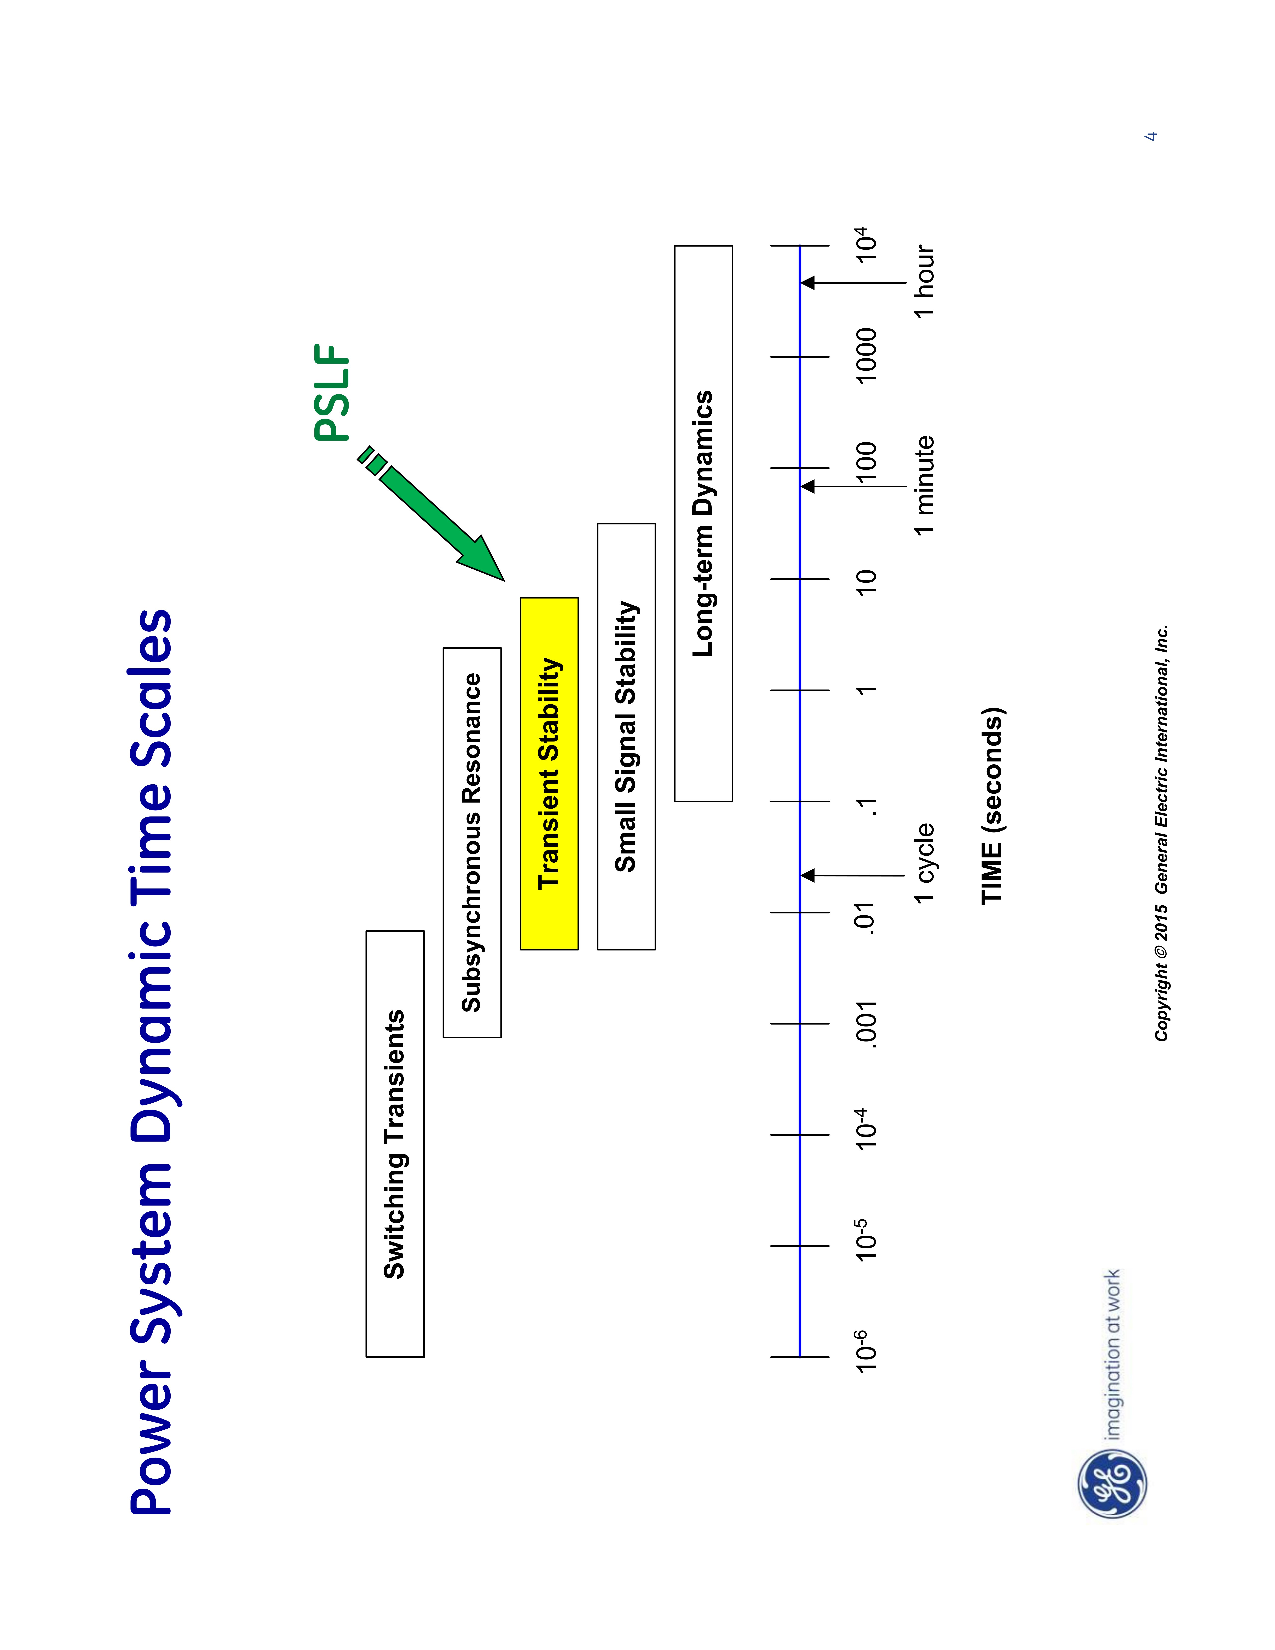
\includegraphics[angle=-90,origin=c,width=1.05\linewidth]{GEtimeScales} 
\end{figure}
\end{frame}

%------------------------------------------------
\section{Assumptions}
\begin{frame}
This simulation assumes:
\begin{enumerate}
	\item Time steps of 0.5 to 1 second.
	\item Fast dynamics are 'mostly' ignored.
	\item System remains stable.
	\item System frequency is described by the combined PU swing equation:
	\setcounter{assumptions}{\value{enumi}} % allow for break in counting
\end{enumerate}
	\[ \dot{\omega}_{sys} = \dfrac{1}{2H_{sys} } \left( \dfrac{P_{acc, sys} }{\omega_{sys}(t)} - D_{sys}\Delta\omega_{sys}(t)  \right)\] 
\begin{enumerate}
	\setcounter{enumi}{\value{assumptions}}
		\item No system damping $(D_{sys} = 0)$.	
\end{enumerate}
\end{frame}
%------------------------------------------------
\section{Project Goals}
\begin{frame}
Project Goals:
\begin{itemize}
	\item Develop computer software for LTD simulations using PSLF systems $(.sav)$, dynamic data $(.dyd)$, and customized dynamic models.
	\item Use software to investigate system reactions that may be impractical to simulate using other approaches.
	\item Write a master's thesis about it.
\end{itemize}

\end{frame}
%------------------------------------------------

%************************************************
\section{Proof of Concept}
%________________________________________________
%------------------------------------------------
\begin{frame}
PSLF test system:
\vspace{-1em}\\
\begin{figure}
	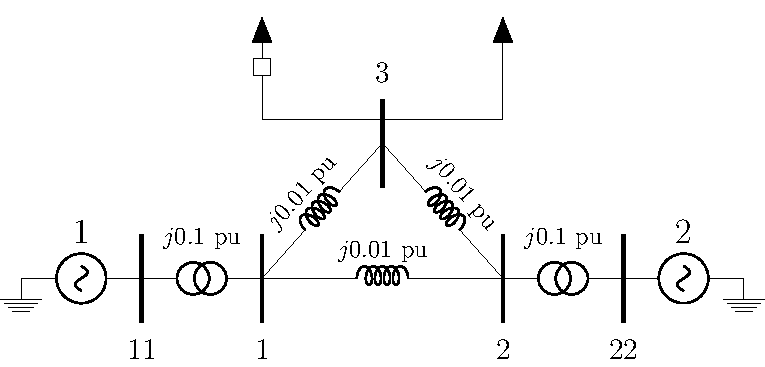
\includegraphics[width=\linewidth]{cicuitEE554}
\end{figure}
\vspace{-1em}
Generators are identical genrou models. \\Gen 1 has a tgov1 governor.
\end{frame}

%------------------------------------------------
\begin{frame}[fragile]
pgov1 : Proportional gain control of $P_M$ \\
\begin{figure}
	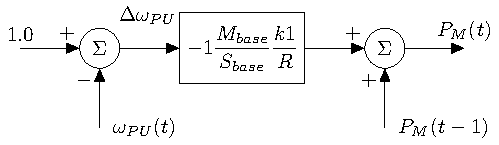
\includegraphics[width=\linewidth]{pgov1}
\end{figure}\vspace{-1em}
Entered into system via parsed text file:
\begin{lstlisting}[frame=single, basicstyle=\footnotesize]
# model  busnum busnam basekv id : #9 mwcap droop
#!pgov1   11 "11" 22.00 "1 " : #9 mwcap=100.0 0.05
\end{lstlisting}\vspace{-0.5em}
\footnotesize Model adapted from [3]
\end{frame}

%________________________________________________
\section{Initial Results}
\subsection{Dynamic model 'pgov1' experiment: +1 MW t=2, -1 MW t=30}
%------------------------------------------------
\begin{frame}
pgov1 on Gen 1, $t_\text{step}=$1.0 second
\begin{figure}
	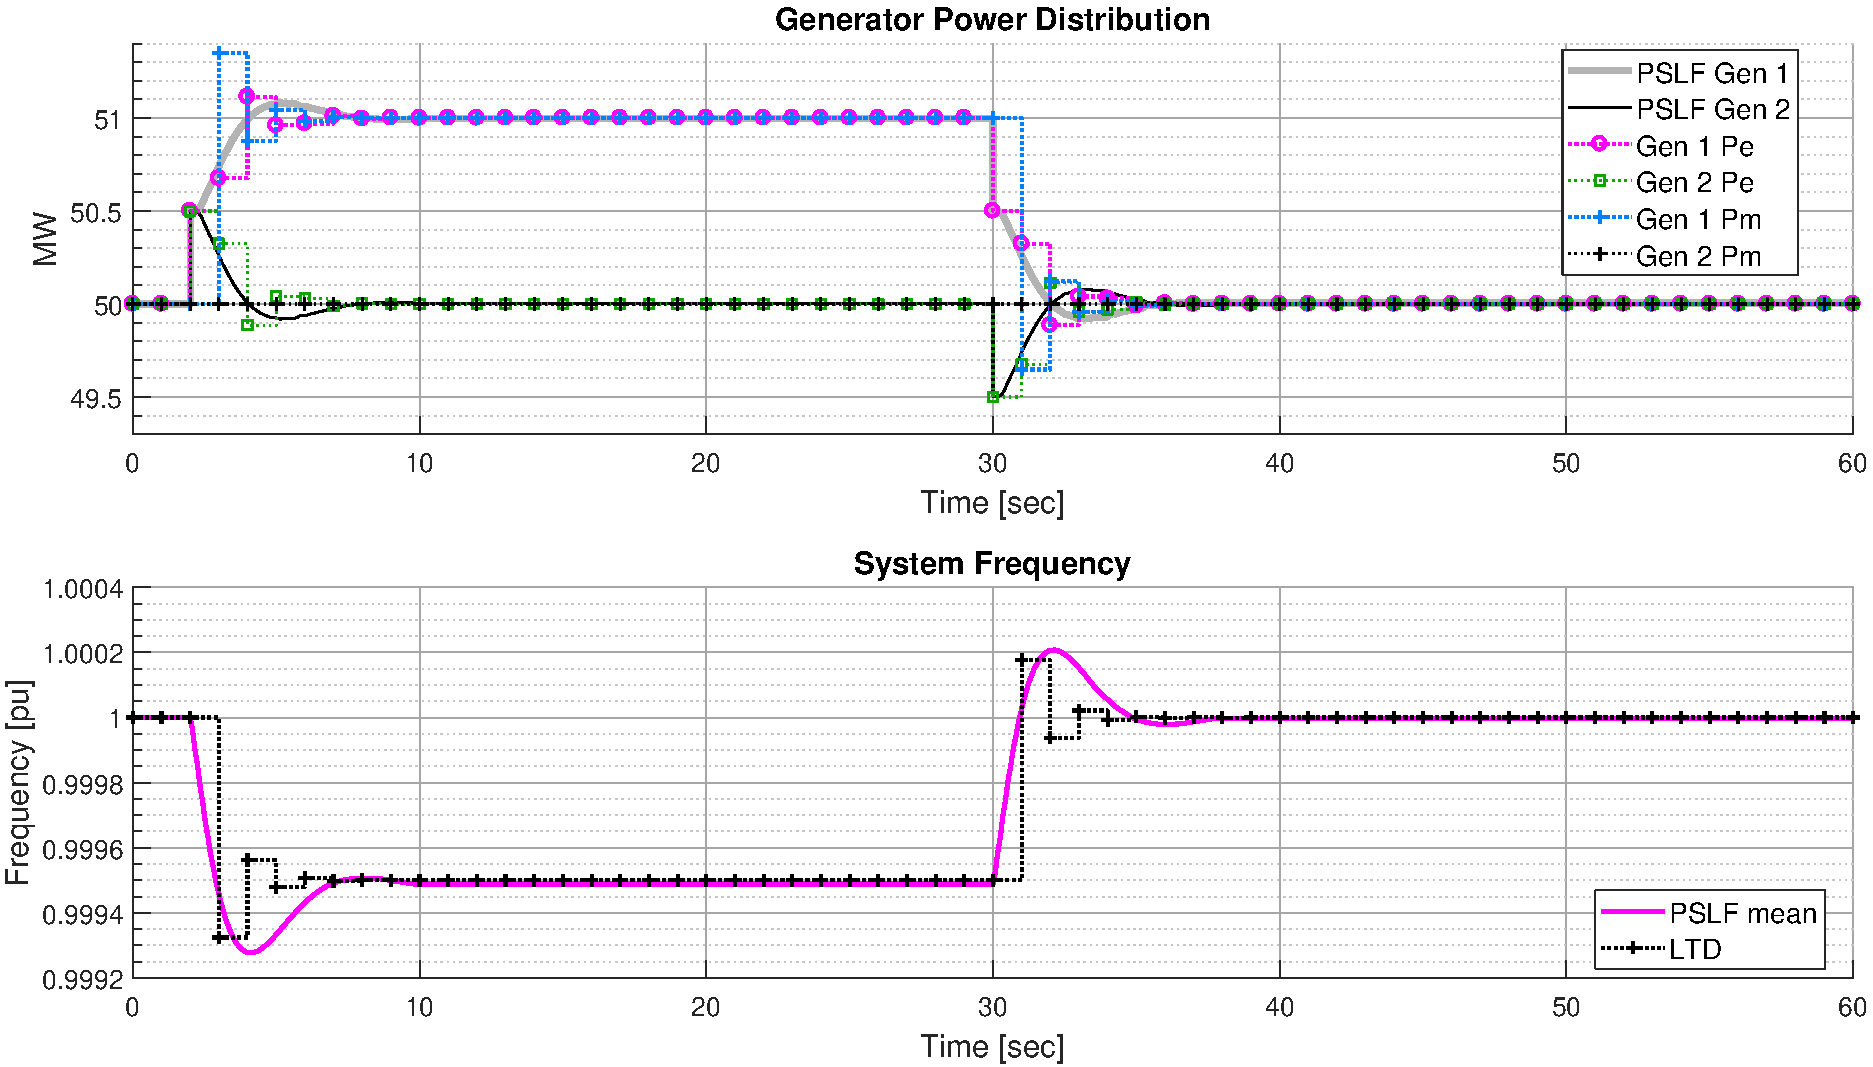
\includegraphics[width=\linewidth]{pgov1IABoneSec}% pgov1C} % this was just lucky results
\end{figure}
\end{frame}
%------------------------------------------------
\begin{frame}
pgov1 on Gen 1, $t_\text{step}=$0.5 second
\begin{figure}
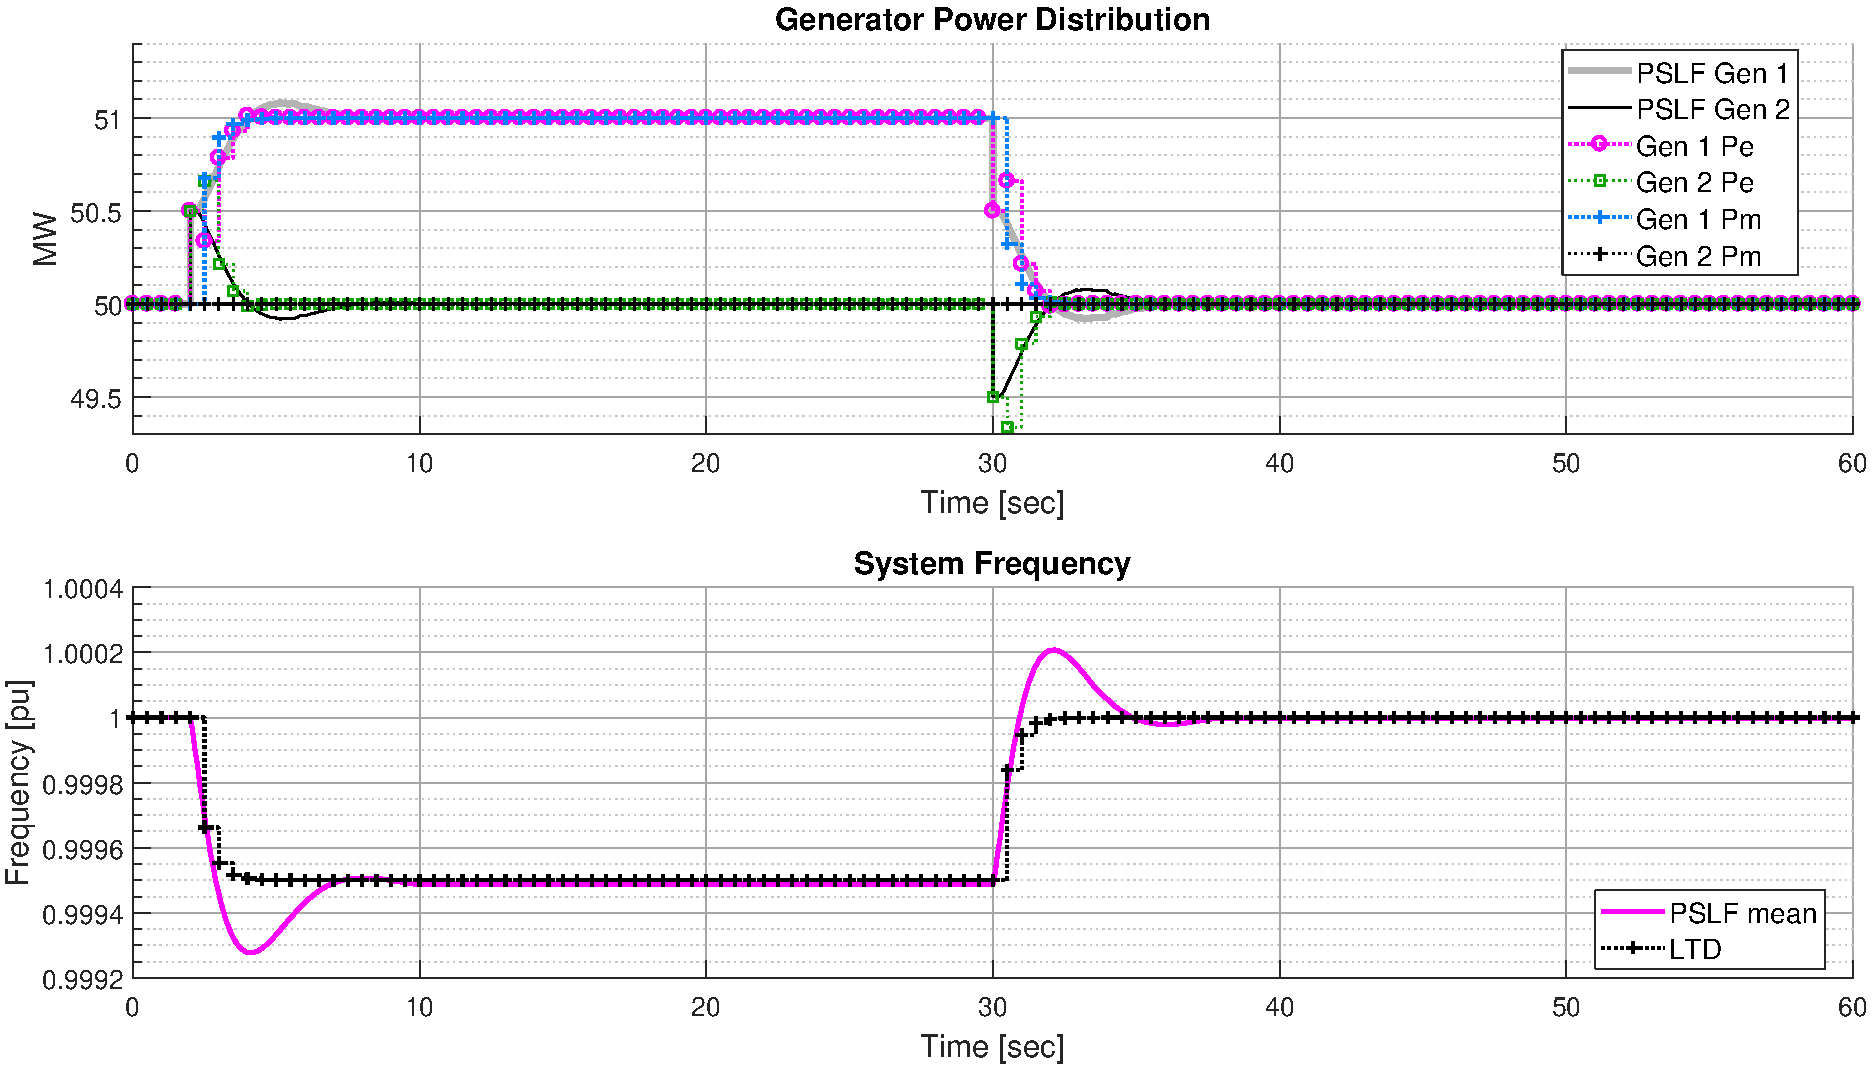
\includegraphics[width=\linewidth]{pgov1IAB2}% pgov1C} % this was just lucky results
\end{figure}
\end{frame}
%------------------------------------------------

\end{document}